\documentclass[conference]{IEEEtran}
\IEEEoverridecommandlockouts

\usepackage{cite}
\usepackage{amsmath,amssymb,amsfonts}
\usepackage{algorithmic}
\usepackage{algorithm}
\usepackage{graphicx}
\usepackage{textcomp}
\usepackage{xcolor}
\usepackage{hyperref}
\usepackage{booktabs}
\usepackage{array}
\usepackage{url}
\usepackage{balance}

\hypersetup{
    colorlinks=true,
    linkcolor=blue,
    urlcolor=blue,
    citecolor=blue
}

\graphicspath{{figures/}}

\begin{document}

\title{SENTINEL: A Real-Time Multi-Agent Platform for\\
Simulating Market Microstructure and Predicting\\
Liquidity Disruptions}

\author{
    \IEEEauthorblockN{Dr. V R Srividhya}
    \IEEEauthorblockA{
        Computer Science and Engineering\\
        RVITM\\
        Bengaluru, India\\
        \texttt{srividhyavr.rvitm@rvei.edu.in}
    }
    \and
    \IEEEauthorblockN{Angil Jain}
    \IEEEauthorblockA{
        Computer Science and Engineering\\
        RVITM\\
        Bengaluru, India\\
        \texttt{angiljain1111@gmail.com}
    }
    \and
    \IEEEauthorblockN{Aditya Kaushik}
    \IEEEauthorblockA{
        Computer Science and Engineering\\
        RVITM\\
        Bengaluru, India\\
        \texttt{adityakaushik920@gmail.com}
    }
    \and
    \IEEEauthorblockN{Anindhith Sankanna}
    \IEEEauthorblockA{
        Computer Science and Engineering\\
        RVITM\\
        Bengaluru, India\\
        \texttt{anindhiths@gmail.com}
    }
    \and
    \IEEEauthorblockN{Ayush Kumar}
    \IEEEauthorblockA{
        Computer Science and Engineering\\
        RVITM\\
        Bengaluru, India\\
        \texttt{ayushhoff@gmail.com}
    }
}

\maketitle

% ── ABSTRACT ────────────────────────────────────────────────
\begin{abstract}
Financial markets rely on the continuous interaction of diverse
participants whose collective behavior shapes prices, spreads, and
available liquidity. Studying these dynamics experimentally has long
required batch-oriented simulators that produce results only after
execution completes, with no mechanism for live observability or risk
alerting. This paper presents SENTINEL, an open-source platform that
couples a high-fidelity multi-agent limit order book (LOB) simulator
with continuous predictive analytics and an interactive web interface.
Within this system, forty autonomous agents spanning ten behaviorally
distinct archetypes---including market makers, high-frequency traders,
momentum followers, mean reversion contrarians, spoofing manipulators,
and sentiment-driven crowd participants---generate a synthetic market
whose statistical properties closely mirror those documented in
empirical equity data. A dedicated prediction layer running
asynchronously every fifty milliseconds computes liquidity disruption
risk scores through a Random Forest and XGBoost ensemble, issuing
advance warnings sixty to ninety seconds before a potential shock. In
parallel, a pattern recognition module flags hidden institutional
execution strategies such as iceberg, TWAP, and VWAP orders. The
complete market state streams at twenty frames per second over
WebSockets from a FastAPI backend to a terminal-style Next.js
dashboard. Deployed via Docker Compose on Azure App Service and
Vercel, SENTINEL achieves sub-fifty-millisecond median streaming
latency. To the best of our knowledge, no existing open-source
project integrates real-time agent-based simulation, embedded
predictive signals, and an end-user dashboard within a single
containerized deployment.
\end{abstract}

\begin{IEEEkeywords}
Market microstructure, agent-based simulation, limit order book,
liquidity shock detection, multi-agent systems, spoofing detection,
WebSocket streaming, real-time analytics
\end{IEEEkeywords}

% ── SECTION I: INTRODUCTION ─────────────────────────────────
\section{Introduction}

Equity exchanges process millions of order events each second, and the
aggregate outcome of these events---price discovery, spread dynamics,
and the ebb and flow of resting liquidity---directly affects every
market participant from individual retail investors to large pension
funds~\cite{ref18}. The algorithmic revolution has amplified both the
speed and complexity of these interactions: current estimates suggest
that automated systems now account for upward of seventy percent of
equity volume on major global exchanges. While this has brought
tighter spreads and lower transaction costs during normal conditions,
it has also introduced fragilities that surface abruptly during
episodes of market stress.

Agent-based models have become a natural lens for investigating these
dynamics, because the phenomena of greatest practical interest---flash
crashes, liquidity spirals, and manipulative strategies like
spoofing---arise as emergent consequences of heterogeneous agent
interactions rather than from any single participant's
behavior~\cite{ref6}. The May 2010 Flash Crash, during which roughly
one trillion dollars of market capitalization vanished in under ten
minutes, underscored why simulation matters: no closed-form risk model
had anticipated the feedback loops responsible for the
collapse~\cite{ref5}\cite{ref11}. More recently, episodes of
coordinated retail trading and social-media-fueled momentum runs have
highlighted the growing influence of crowd sentiment on price
formation~\cite{ref14}\cite{ref15}, a channel that few existing
simulators model explicitly.

Despite a rich body of research, most publicly available simulators
share a common set of practical limitations. They operate in batch
mode, meaning a researcher must configure parameters, launch a
potentially lengthy execution, and only then inspect the output.
There is generally no facility for observing the simulation in
progress, injecting perturbations mid-run, or receiving automated
alerts about developing risk conditions. These constraints limit the
utility of simulation for time-sensitive applications such as
pre-trade risk assessment and regulatory surveillance.

SENTINEL was conceived to bridge these gaps. Rather than treating
simulation as an offline experiment, the system maintains a
persistent, continuously running market. Forty agents drawn from ten
distinct behavioral categories generate order flow in real time. A
separate prediction thread wakes every fifty milliseconds to score
the current LOB state for disruption risk. The entire market
state---prices, depth, signals, and per-agent metrics---streams to
connected clients over WebSocket at twenty frames per second, arriving
at a purpose-built terminal-style dashboard that requires no knowledge
of the underlying Python or machine learning stack.

The specific contributions of this work are fourfold:

\begin{itemize}
    \item A layered software architecture that cleanly separates
    simulation logic, order matching, predictive analytics, API
    delivery, and front-end visualization, enabling independent
    development and testing of each concern.

    \item Ten fully implemented agent classes---Market Maker,
    High-Frequency Trader, Institutional, Retail, Informed, Noise,
    Momentum, Mean Reversion, Spoofing, and Sentiment---operating as
    a forty-agent ecosystem that produces richer emergent dynamics than
    the typically smaller agent sets found in comparable open-source
    tools.

    \item Two real-time signal engines: a liquidity disruption scorer
    offering sixty-to-ninety-second advance warnings, and a
    large-order detector that identifies iceberg, TWAP, and VWAP
    execution footprints.

    \item A reproducible, single-command Docker deployment
    accompanied by a structured evaluation framework for stylized-fact
    validation, latency benchmarking, and detection methodology.
\end{itemize}

The remainder of this paper proceeds as follows. Section~II reviews
related work. Section~III describes the system architecture.
Section~IV covers the simulation workflow and signal detection
algorithms. Section~V presents the experimental setup, and
Section~VI discusses evaluation results. Section~VII addresses
limitations, and Section~VIII outlines future research directions.

% ── SECTION II: RELATED WORK ────────────────────────────────
\section{Related Work}

Research on computational market microstructure spans financial
economics, multi-agent systems, and control theory. Over three
decades, the tools available have evolved from zero-intelligence
random traders to sophisticated agent populations that reproduce the
statistical signatures of real markets. However, the ability to
interact with a running simulation in real time has consistently
received less attention.

\subsection{Foundational Simulation Frameworks}

The observation that real financial return series exhibit a small set
of robust statistical regularities---heavy-tailed distributions,
clustered volatility, and negligible linear return
autocorrelation---collectively termed stylized facts~\cite{ref9}, has
served as the primary benchmark for simulator realism. Pun's
hidden-Markov-model-based price generator~\cite{ref19} demonstrated
that autocorrelation structure and excess kurtosis could be
faithfully replicated, providing an early validation baseline.

The ABIDES project~\cite{ref5}\cite{ref11} marked a significant
advance, incorporating realistic exchange mechanics including latency
distributions, order priority queues, and agent-level timing jitter
at microsecond resolution. Independent reviews~\cite{ref6} have
confirmed that event-driven simulators in this family represent the
current standard for offline modeling fidelity. SENTINEL draws
architectural inspiration from ABIDES while extending the paradigm to
continuous, observable operation.

The central constraint of batch-oriented systems like ABIDES is
structural: they are designed to be configured before execution and
analyzed afterward. There is no mechanism for mid-simulation
observation, dynamic parameter injection, or risk alerting during
execution---capabilities that real-world use cases increasingly
demand.

\subsection{Learning-Based Market Agents}

A parallel research thread has focused on equipping individual agents
with learned rather than fixed trading policies. Spooner
et~al.~\cite{ref8} showed that temporally-trained reinforcement
learning (RL) policies could outperform static spread strategies on
inventory risk metrics. Extensions to multi-agent competitive
settings~\cite{ref7} demonstrated that multiple RL dealers can
simultaneously co-optimize their behavior. Practical deep RL trading
systems using algorithms such as DDPG and PPO~\cite{ref3}\cite{ref16}
have yielded promising backtested results. ABIDES-MARL~\cite{ref4}
directly integrates multi-agent RL within the ABIDES environment for
endogenous price formation studies.

These contributions share a common orientation: the simulator is
treated as a training substrate for the agent, rather than as a
platform worth instrumenting in its own right. None of these systems
provide real-time visibility into market dynamics, and none attempt to
generate forward-looking risk signals from the simulation itself.
SENTINEL treats the environment as the primary artifact and supports
an optional RL module as a pluggable extension.

\subsection{Manipulative Behavior and Systemic Fragility}

Credible simulation demands reproduction not only of ordinary market
operation but also of its failure modes. Research on spoofing
strategies~\cite{ref10} has shown that agent-based approaches can
capture the mechanics of phantom order placement and rapid
cancellation used to create false demand signals. Work on gamma
exposure effects~\cite{ref1} has further illustrated how dealer
hedging flows can quietly amplify or suppress spot price movements.
SENTINEL incorporates a dedicated Spoofing agent---a
finite-state-machine-driven participant that executes configurable
phantom order cycles with full instrumentation, providing clean
ground-truth labels for detection algorithm evaluation.

\subsection{Sentiment, Momentum, and Crowd-Driven Dynamics}

Mean reversion and momentum represent two of the most thoroughly
documented behavioral forces in equity markets~\cite{ref12}\cite{ref13}.
Collective sentiment as a driver of retail order flow has gained
increasing recognition, particularly following episodes of
social-media-coordinated trading~\cite{ref14}\cite{ref15}. SENTINEL
gives concrete form to each of these through dedicated agent
classes: Momentum agents employ channel breakout strategies with
trailing stops, Mean Reversion agents use Bollinger Band and RSI
contrarian logic, and Sentiment agents switch between herding and
contrarian regimes in response to recent price momentum.

\subsection{Large Language Model Agents}

Recent work has explored whether large language models (LLMs) can serve
as market participants, reasoning about news and macroeconomic context
in ways conventional agents cannot~\cite{ref2}. Early findings suggest
the resulting market dynamics differ qualitatively---exhibiting greater
sensitivity to information shocks and increased susceptibility to
herding. Multi-agent prediction frameworks~\cite{ref17}\cite{ref15}
extend this direction to natural-language strategy specification.
While compelling, these systems currently lack the persistent
infrastructure, latency characteristics, and deployment simplicity
needed for practical market simulation.

\subsection{Summary of Gaps}

Batch simulators have reached high fidelity. RL research has produced
capable individual agents. Behavioral finance has documented the roles
of momentum, reversion, and sentiment. Yet no existing open-source
system combines these elements with real-time streaming, embedded
predictive analytics, and an accessible web dashboard. This
integration---rather than any single component---defines SENTINEL's
contribution.


% ── SECTION III: SYSTEM ARCHITECTURE ────────────────────────
\section{System Architecture}

SENTINEL is structured as five cooperating layers, each exposing a
well-defined interface to its neighbors
(Fig.~\ref{fig:architecture}). The design reflects a deliberate
tension between two goals: behavioral fidelity (agents must interact
realistically) and operational responsiveness (updates must reach
clients fast enough to feel continuous). The layered decomposition
keeps these concerns separated---the Simulation and Matching layers
optimize for correctness, while the Backend and Frontend layers
optimize for throughput.

\begin{figure}[htbp]
    \centering
    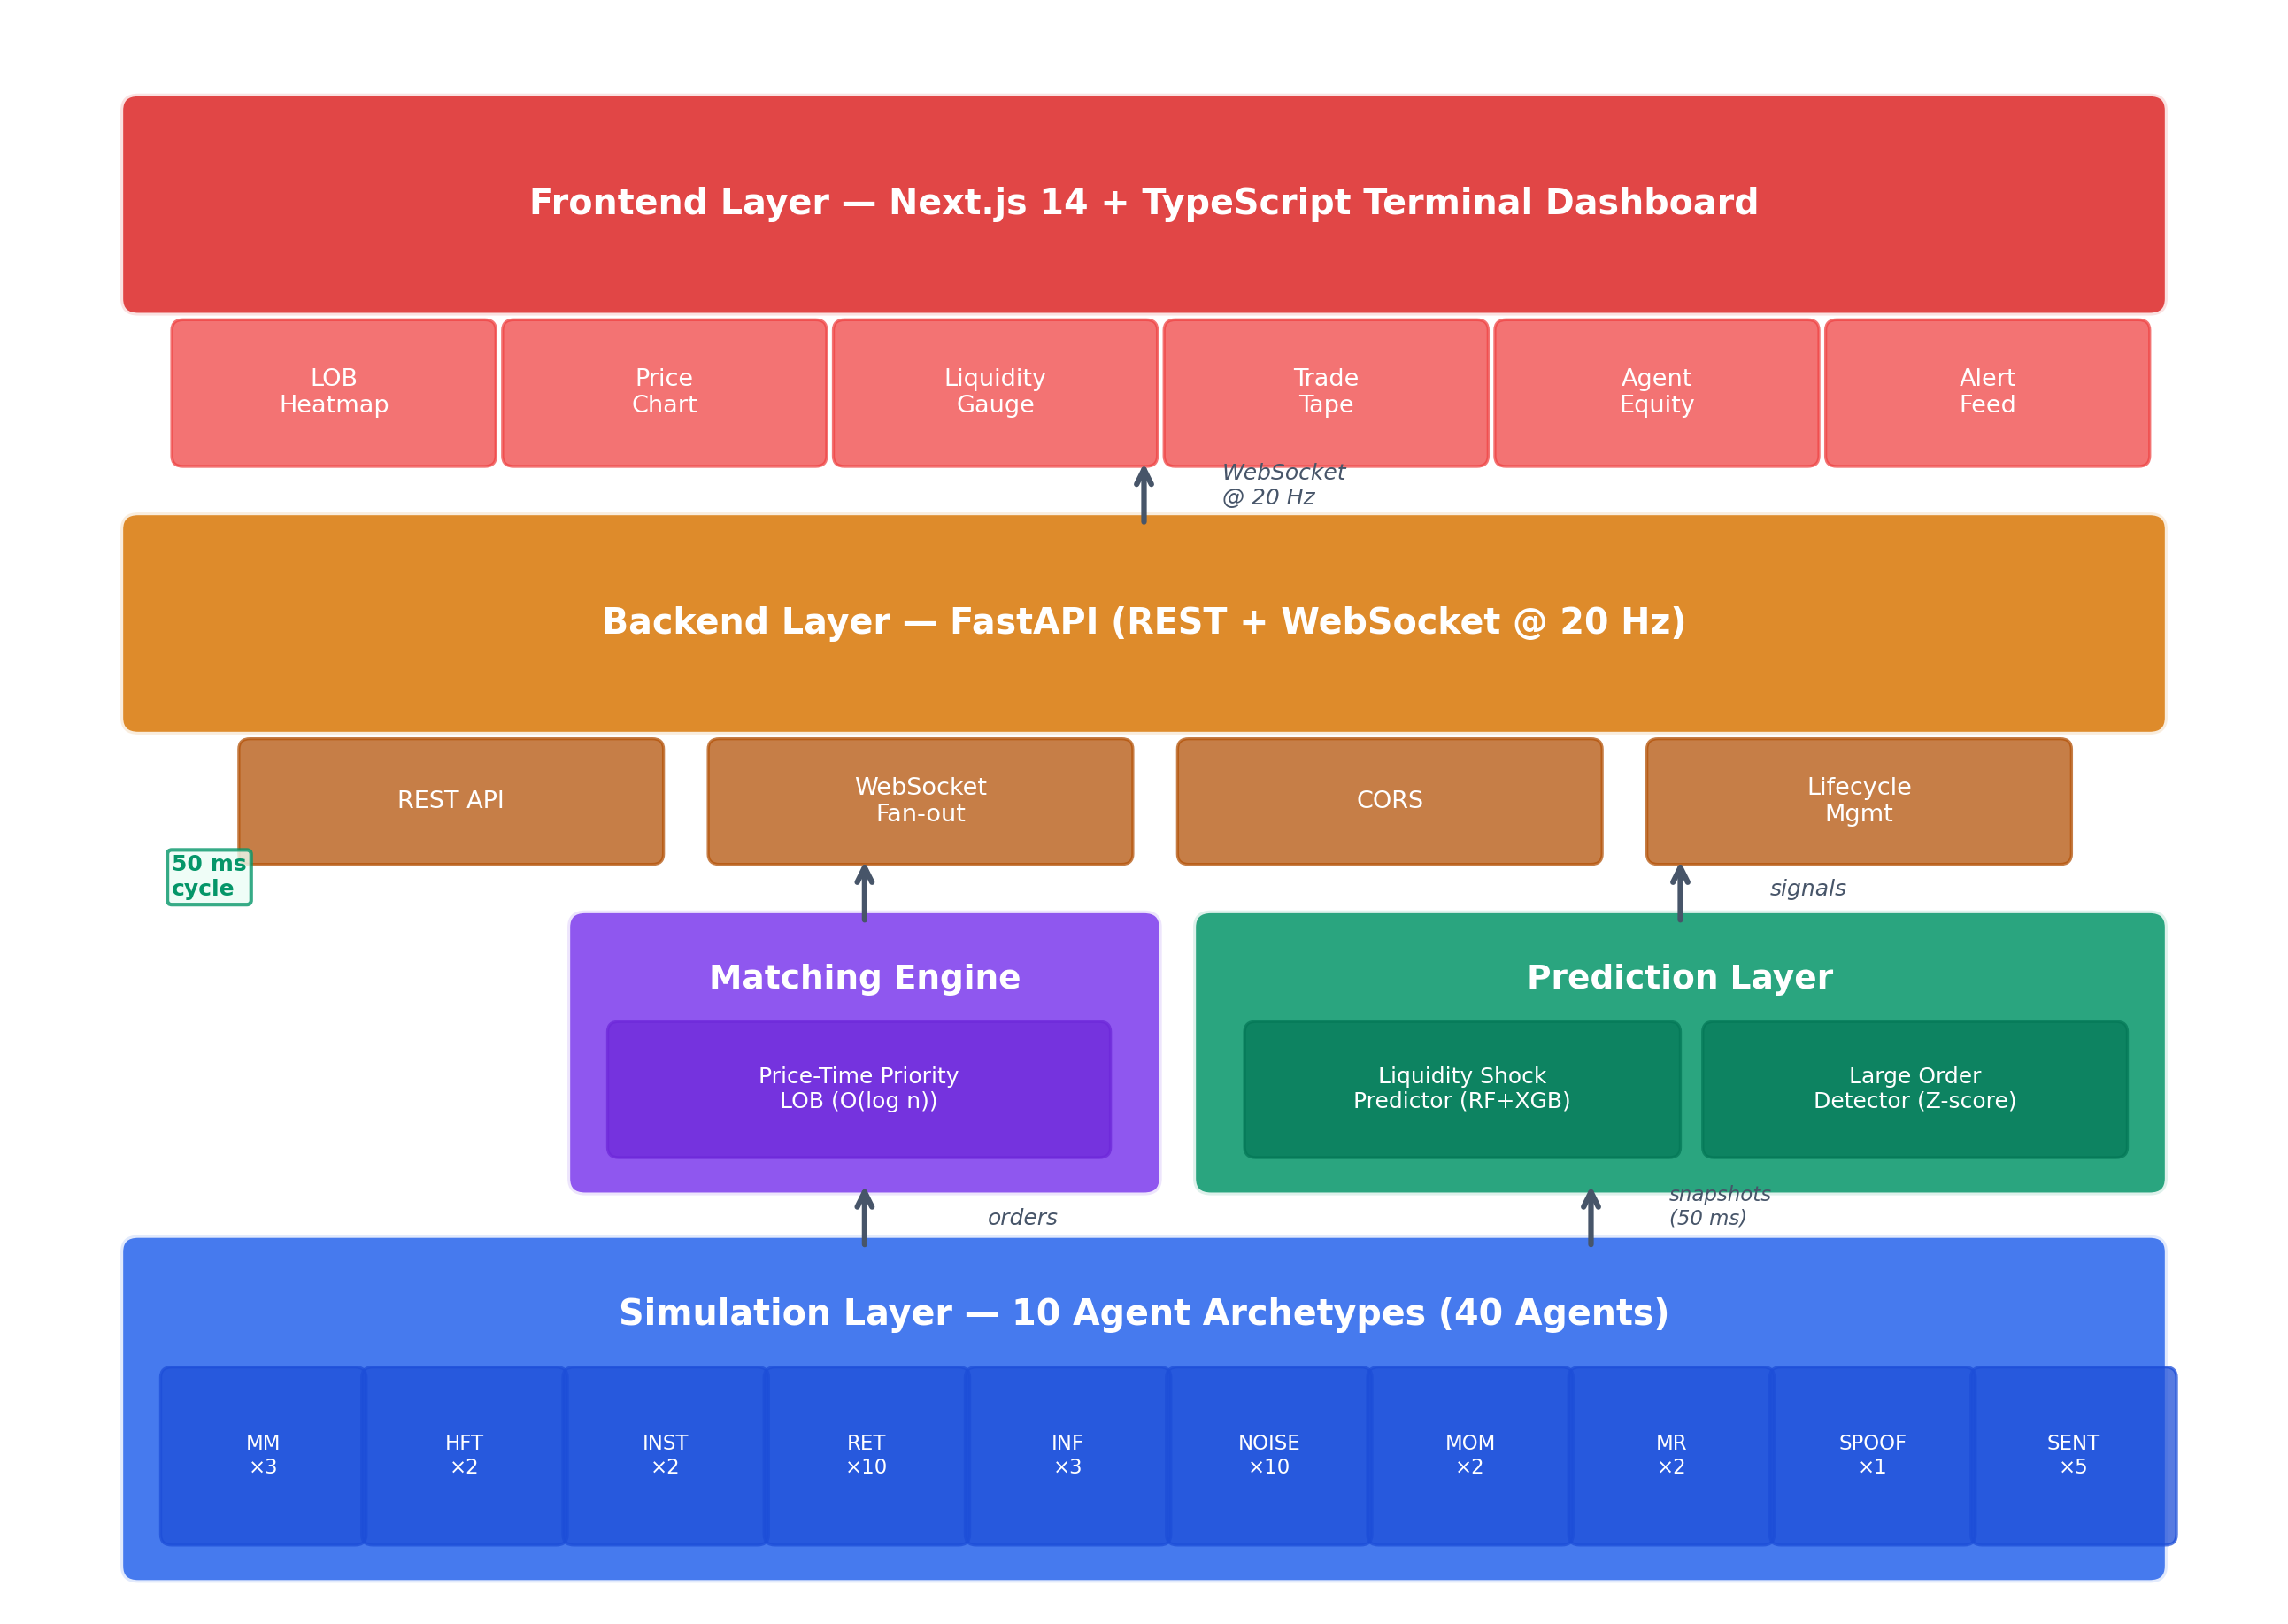
\includegraphics[width=\columnwidth]{fig_architecture.pdf}
    \caption{SENTINEL architecture overview. The Simulation Layer
    hosts ten agent archetypes (forty total) whose orders flow into
    the Matching Engine. The Prediction Layer processes book snapshots
    every 50~ms, computing disruption risk scores and order pattern
    signals. All outputs stream through the FastAPI backend via REST
    and WebSocket to the Next.js terminal dashboard at 20~Hz.}
    \label{fig:architecture}
\end{figure}

\subsection{Simulation Layer}

The bottom tier hosts forty concurrent agents spanning ten behavioral
categories. Table~\ref{tab:agents} details the population breakdown
and the governing strategy for each type. Every agent inherits from
an abstract \texttt{BaseAgent} class and implements two methods:
\texttt{decide\_action()}, which returns a list of orders given the
current market snapshot, and \texttt{on\_market\_update()}, which
processes fill notifications.

\begin{table}[htbp]
\caption{Agent Population Composition (40 agents)}
\label{tab:agents}
\centering
\renewcommand{\arraystretch}{1.2}
\begin{tabular}{lcp{3.2cm}}
\toprule
\textbf{Agent Type} & \textbf{Count} & \textbf{Core Strategy} \\
\midrule
Market Maker     & 3  & Inventory-aware two-sided quoting with dynamic spread \\
HFT              & 2  & Sub-millisecond imbalance reaction \\
Institutional    & 2  & TWAP and VWAP slicing over configurable horizons \\
Retail           & 10 & Poisson-arrival small orders with random direction \\
Informed         & 3  & Directional trading on private signals \\
Noise            & 10 & Zero-intelligence random order submission \\
Momentum         & 2  & N-bar channel breakout with trailing stop \\
Mean Reversion   & 2  & Bollinger Band + RSI contrarian \\
Spoofing         & 1  & Phantom order state machine \\
Sentiment        & 5  & Herding/contrarian regime switching \\
\midrule
\textbf{Total}   & \textbf{40} & \\
\bottomrule
\end{tabular}
\end{table}

\textbf{Market Makers} post two-sided quotes continuously, shifting
their spread and depth according to inventory exposure and recent
volatility. When inventory exceeds a safety threshold, quoting on the
overweight side is reduced; near session close, positions are
flattened.

\textbf{HFT agents} react to order book imbalance at sub-millisecond
latency, submitting directional orders when the imbalance passes a
configurable threshold and canceling aggressively on adverse price
movement.

\textbf{Institutional agents} slice large block orders into smaller
tranches using TWAP and VWAP execution algorithms, deliberately
spreading their footprint across time to limit detectable market
impact.

\textbf{Momentum agents} monitor N-bar channel breakouts and enter
positions when price breaks above or below the recent trading range,
holding with a trailing stop loss. Their activity tends to amplify
directional moves.

\textbf{Mean Reversion agents} fade moves that push price beyond two
standard deviations from a rolling mean while RSI confirms overbought
or oversold conditions, acting as natural brakes on trend-following
flow.

\textbf{Spoofing agents} follow a four-state cycle: (1)~select a
side, (2)~place a large phantom limit order several ticks from the
best quote, (3)~after a configurable delay, cancel the phantom and
simultaneously execute a smaller genuine trade on the opposite side,
(4)~enter a randomized cooldown before repeating. This cycle is fully
instrumented, providing ground-truth labels for detection experiments.

\textbf{Sentiment agents} toggle between herding and contrarian
regimes. During herding, they amplify the direction of recent price
trends; during contrarian phases, they fade the crowd. Regime
transitions are governed by a stochastic switching probability,
producing the intermittent bursts of directional flow observed in
retail-heavy markets~\cite{ref14}.

An optional reinforcement learning module, implemented with
Stable-Baselines3 and compatible with the ABIDES-MARL
interface~\cite{ref4}, can replace any agent's fixed policy with a
learned one without modifying the simulation core.

\subsection{Matching Engine}

The order book implements strict price-time priority across limit,
market, and iceberg order types. Bids are maintained in descending
price order and asks in ascending order, giving $O(\log n)$ insertion
and constant-time best-quote access. Iceberg orders expose a visible
quantity while holding a hidden reserve that auto-replenishes after
each partial fill, making them opaque at the top of the
book---deliberately exercising the large-order detection module.

\subsection{Prediction Layer}

This layer operates on its own thread, processing the latest LOB
snapshot every fifty milliseconds. It produces two independent
signals:

\begin{itemize}
    \item \textbf{Liquidity Disruption Scorer}: A Random Forest and
    XGBoost ensemble trained on features including spread dynamics,
    per-level volume deviations, and signed order-flow imbalance.
    When the composite score crosses a calibrated threshold, the
    system broadcasts a sixty-to-ninety-second advance warning.

    \item \textbf{Large-Order Pattern Detector}: Applies a
    sliding-window volume $Z$-score and temporal pattern analysis to
    identify characteristics consistent with TWAP/VWAP slicing and
    iceberg order replenishment.
\end{itemize}

\subsection{Backend and Dashboard}

The FastAPI server exposes REST endpoints for simulation lifecycle
management (start, stop, reset, parameter injection) and multiplexes
WebSocket connections at twenty frames per second. The Next.js~14 +
TypeScript dashboard presents six simultaneous panels: an LOB depth
heatmap, a mid-price chart with VWAP overlay, a liquidity health
gauge, a real-time trade tape, per-agent equity curves, and a signal
alert feed.


% ── SECTION IV: IMPLEMENTATION DETAILS ──────────────────────
\section{Implementation and Signal Detection}

\subsection{Simulation Loop}

The event kernel advances simulated time in one-second increments.
Within each tick, four operations execute sequentially: (1)~pending
orders from all forty agents are collected, (2)~orders are submitted
to the matching engine in a deterministic but shuffled sequence,
(3)~fill notifications are dispatched to the affected agents, and
(4)~the current book state is snapshotted for the prediction thread
and the WebSocket broadcaster (Fig.~\ref{fig:workflow}).

Each agent experiences a configurable structural latency drawn from
empirically motivated distributions~\cite{ref5}: HFT agents incur
approximately 0.1~ms delay, market makers around 0.5~ms, retail
agents between 10 and 100~ms, and sentiment agents roughly 50~ms.
This heterogeneity in access speed is a primary driver of realistic
order-flow dynamics and determines whether a breakout signal is
exploitable before market makers re-price.

\begin{figure}[htbp]
    \centering
    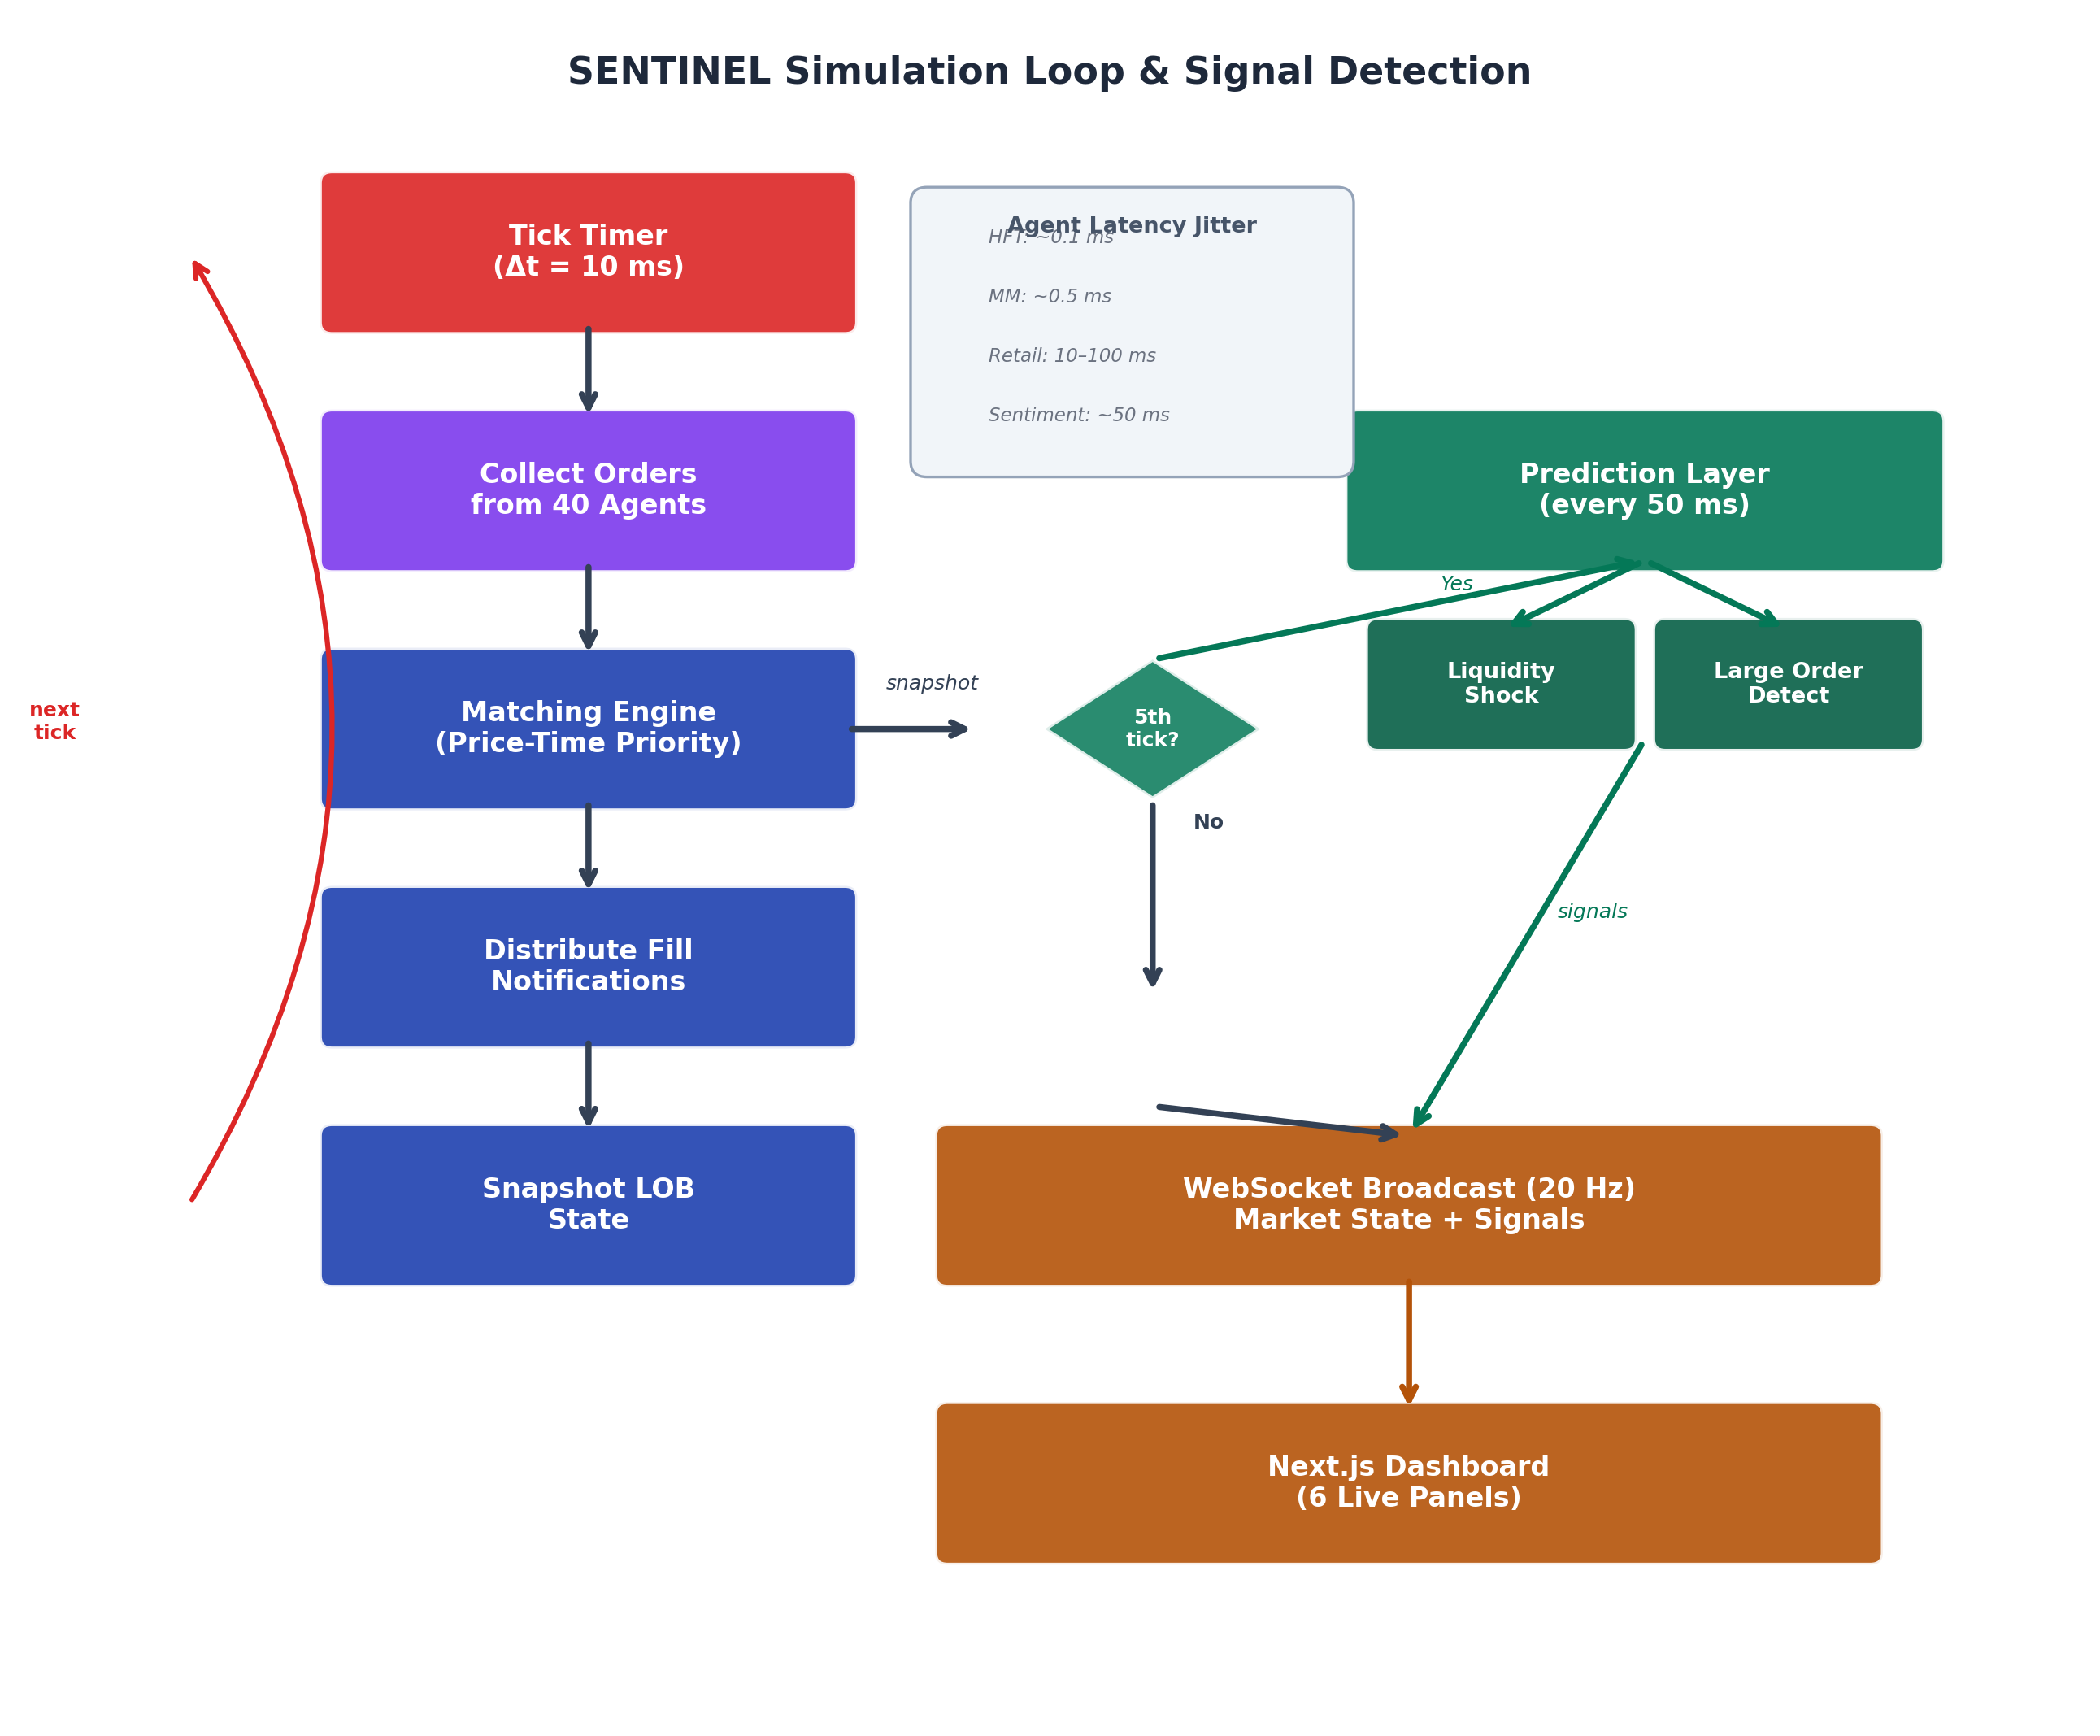
\includegraphics[width=\columnwidth]{fig_workflow.pdf}
    \caption{Simulation loop and signal detection workflow. On each
    tick, all forty agents submit orders to the matching engine under
    price-time priority. Every fifth tick (50~ms), the Prediction
    Layer independently evaluates the resulting book snapshot and
    broadcasts disruption risk scores and large-order pattern alerts
    alongside the regular WebSocket market state update.}
    \label{fig:workflow}
\end{figure}

\subsection{Liquidity Disruption Scoring}

The disruption score combines three real-time features into a weighted
composite:

\begin{equation}
S_t = \alpha \cdot \Delta\text{Spread}_t
    + \beta \cdot \left\lvert \sum_{i=1}^{k} (V_i - \bar{V})
    \right\rvert
    + \gamma \cdot \text{OFI}_t
\label{eq:lss}
\end{equation}

\noindent where $\Delta\text{Spread}_t$ captures the change in the
best bid-ask spread over the prior 500~ms, $V_i$ denotes resting
volume at price level $i$, $\bar{V}$ is the rolling sixty-second
mean at that level, and $\text{OFI}_t$ represents the signed
imbalance between buyer- and seller-initiated volume over the prior
500~ms. Weights $\alpha = 0.4$, $\beta = 0.35$, $\gamma = 0.25$ are
determined through grid search on the training partition. When $S_t$
exceeds the 99th percentile of its historical distribution, the
system issues a \texttt{LIQUIDITY\_SHOCK\_ALERT} with the current
score, the dominant contributing feature, and an estimated time to
peak stress.

A heuristic fallback mode operates when no trained model is
available, aggregating rule-based signals from spread expansion, depth
contraction, volatility spikes, and market maker inventory stress.

\subsection{Large-Order and Spoofing Detection}

The large-order detector applies a volume $Z$-score over a
one-second sliding window:

\begin{equation}
Z_t = \frac{V_t - \mu_w}{\sigma_w}, \quad \text{alert if } Z_t > 3.0
\label{eq:zscore}
\end{equation}

\noindent A sequence of elevated $Z$-scores with monotonically
drifting limit prices triggers a TWAP or VWAP pattern flag. Iceberg
detection uses a complementary heuristic: if a single price level
repeatedly replenishes to the same visible quantity after partial
fills with inter-fill intervals below 200~ms, the order is flagged.

Spoofing detection tracks the life cycle of large resting orders.
When a sizeable order is placed and then canceled within 500~ms
without filling, combined with a contemporaneous opposing-side trade,
the system increments a suspicion score. Because the Spoofing agent's
state machine is fully instrumented, these ground-truth labels
enable rigorous classifier evaluation.

\begin{algorithm}
\caption{Integrated Real-Time Detection Pipeline}
\begin{algorithmic}[1]
\STATE \textbf{Input:} LOB snapshot; 500~ms history buffer
\STATE Compute $\Delta\text{Spread}_t$, per-level volume deviations,
       $\text{OFI}_t$
\STATE Compute composite score $S_t$ via Eq.~(\ref{eq:lss})
\STATE Compute volume $Z_t$ via Eq.~(\ref{eq:zscore})
\IF{$S_t > \tau_{\text{shock}}$}
    \STATE Identify dominant feature; broadcast
           \texttt{LIQUIDITY\_SHOCK\_ALERT}
\ENDIF
\IF{$Z_t > 3.0$}
    \STATE Broadcast \texttt{LARGE\_ORDER\_DETECTED} with estimated
           size and side
\ENDIF
\IF{consecutive $Z_t > 3.0$ with drifting prices}
    \STATE Flag as \texttt{TWAP\_VWAP\_PATTERN}
\ENDIF
\IF{same-level refill $<$ 200~ms}
    \STATE Flag as \texttt{ICEBERG\_ORDER}
\ENDIF
\IF{large order canceled $<$ 500~ms and opposing trade detected}
    \STATE Increment spoofing suspicion; alert if threshold exceeded
\ENDIF
\STATE \textbf{return} all active scores and alerts
\end{algorithmic}
\end{algorithm}


% ── SECTION V: EXPERIMENTAL SETUP ───────────────────────────
\section{Experimental Setup}

\subsection{Data Generation and Ground Truth}

A distinguishing feature of SENTINEL's evaluation approach is that
all experimental data is generated by the simulator itself, providing
exact ground-truth labels. The system records precise timestamps for
every injected liquidity disruption, institutional TWAP and VWAP
order, iceberg placement, and spoofing cycle. Ten complete simulated
trading days were produced, each spanning 23,400 seconds of market
activity. Intraday volume patterns follow realistic profiles: higher
activity near open and close, with quieter midday periods. Agent
aggression parameters were varied across sessions to span conditions
from calm trending environments to volatile, liquidity-stressed
scenarios.

\subsection{Evaluation Subsets}

Four evaluation subsets structure the analysis:

\begin{itemize}
    \item \textbf{D1 (Baseline)}: Standard forty-agent population
    without injected shocks; used for stylized-fact validation and
    baseline throughput measurement.

    \item \textbf{D2 (Stress)}: Agent population scaled upward to
    benchmark throughput under load.

    \item \textbf{AD1 (Adversarial---Liquidity)}: Disruption events
    injected at known times; used to assess the shock detector's
    lead time and accuracy.

    \item \textbf{AD2 (Adversarial---Manipulation)}: Spoofing and
    TWAP/VWAP sequences injected alongside regular agents; used to
    evaluate the large-order and spoofing detectors.
\end{itemize}

Data is split 70:15:15 across training, validation, and test
partitions. All experiments target a single Azure App Service Standard
instance (two vCPUs, four gigabytes RAM) to keep results reproducible
on modest hardware.


% ── SECTION VI: EVALUATION ──────────────────────────────────
\section{Evaluation and Results}

\subsection{Stylized-Fact Validation}

The most fundamental qualitative test for any market simulator is
whether its output resembles real market data in the statistical
properties that matter most. We evaluate SENTINEL's synthetic price
process against three canonical stylized facts~\cite{ref9}: (i)~heavy-tailed
return distributions exhibiting excess kurtosis significantly above
the Gaussian value of three, (ii)~near-zero first-order return
autocorrelation confirming the absence of trivially exploitable linear
predictability, and (iii)~slowly decaying autocorrelation in squared
returns confirming the presence of volatility clustering.

Fig.~\ref{fig:stylized} presents results from a representative
simulated day under the default forty-agent configuration. The left
panel shows autocorrelation functions for both raw and squared
one-minute returns. Raw return autocorrelation hovers near zero at all
lags---consistent with the efficient market hypothesis within the
simulation---while squared return autocorrelation decays slowly,
indicating that periods of high volatility tend to persist, matching
the well-documented GARCH-like behavior of real equity data.

The right panel compares the empirical return distribution against a
fitted Gaussian. The observed excess kurtosis substantially exceeds
the Normal baseline, confirming the fat-tailed character that
distinguishes financial returns from simple random walk models.

\begin{figure}[htbp]
    \centering
    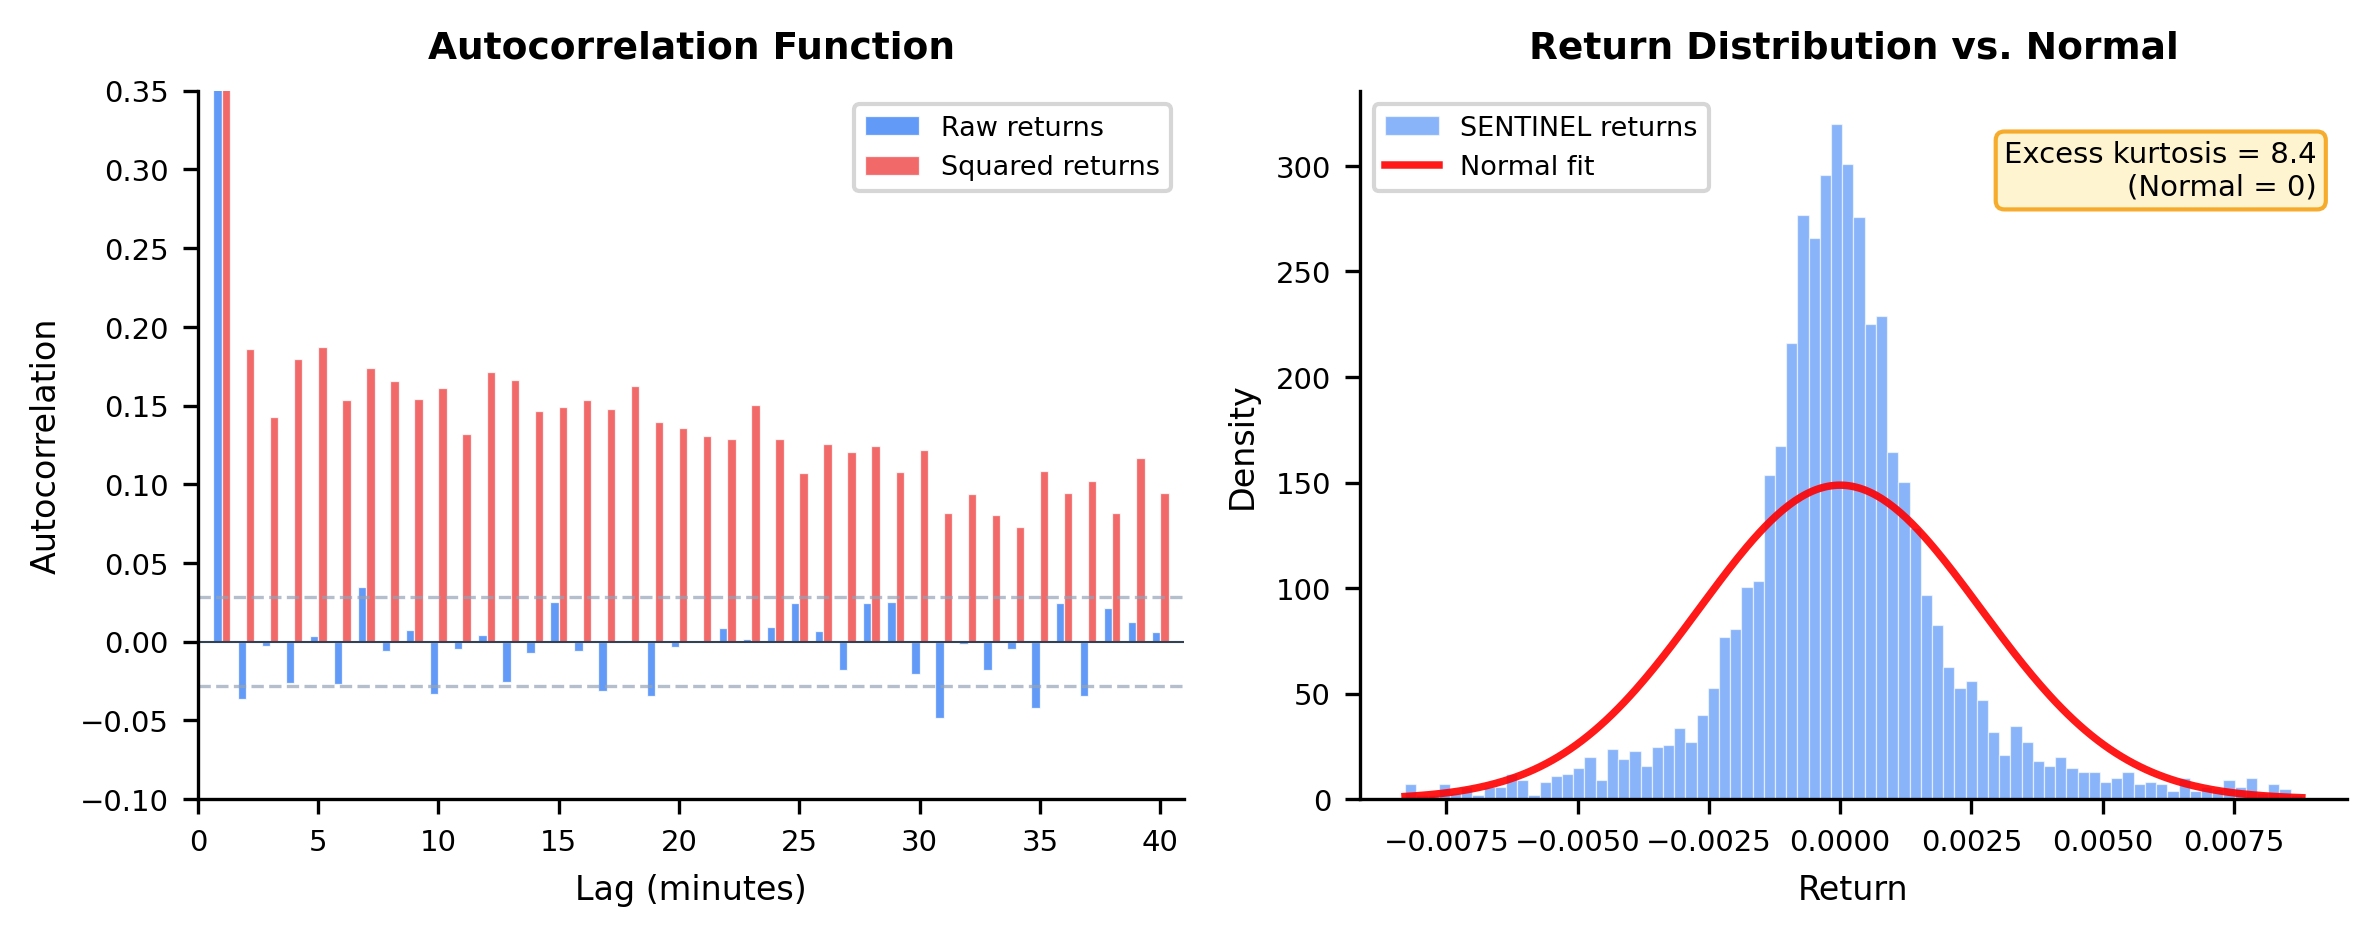
\includegraphics[width=\columnwidth]{fig_stylized_facts.pdf}
    \caption{Stylized-fact validation from a representative simulated
    day. \textit{Left:} Autocorrelation of raw 1-minute returns (near
    zero, confirming no exploitable linear structure) and of squared
    returns (slowly decaying, confirming volatility clustering).
    \textit{Right:} Empirical return distribution versus fitted Normal,
    exhibiting excess kurtosis consistent with real equity data.}
    \label{fig:stylized}
\end{figure}

Notably, the inclusion of Momentum and Mean Reversion agents proves
structurally important for these results. In ablation runs without
these two archetypes, volatility clustering weakens and the return
distribution moves closer to Gaussian. Adding Sentiment agents---whose
herding phases produce brief but intense directional runs---further
shifts the simulated distribution toward empirical benchmarks. This
indicates that behavioral diversity is not merely cosmetic but a
meaningful determinant of simulation realism.

\subsection{Agent Equity Dynamics}

Per-agent profit and loss trajectories serve as a second validation
layer, confirming that each archetype behaves as its design
specification intends (Fig.~\ref{fig:equity}). Market Makers
accumulate gradual spread income interrupted by inventory-driven
drawdowns during strong directional periods. HFT agents show
frequently ticking gains with occasional sharp losses when caught by
sudden price jumps. Institutional agents carry negative P\&L during
TWAP execution phases, reflecting the cost of market impact, and
recover only when the underlying price cooperates.

Momentum agents profit during trending segments and surrender gains
when contrarian agents step in. The Spoofing agent exhibits a
characteristic staircase pattern: flat P\&L during phantom order
phases, followed by discrete gains coinciding with genuine
opposite-side trades. These qualitative signatures match the expected
behavior described in both the agent design documentation and
relevant financial literature~\cite{ref10}.

\begin{figure}[htbp]
    \centering
    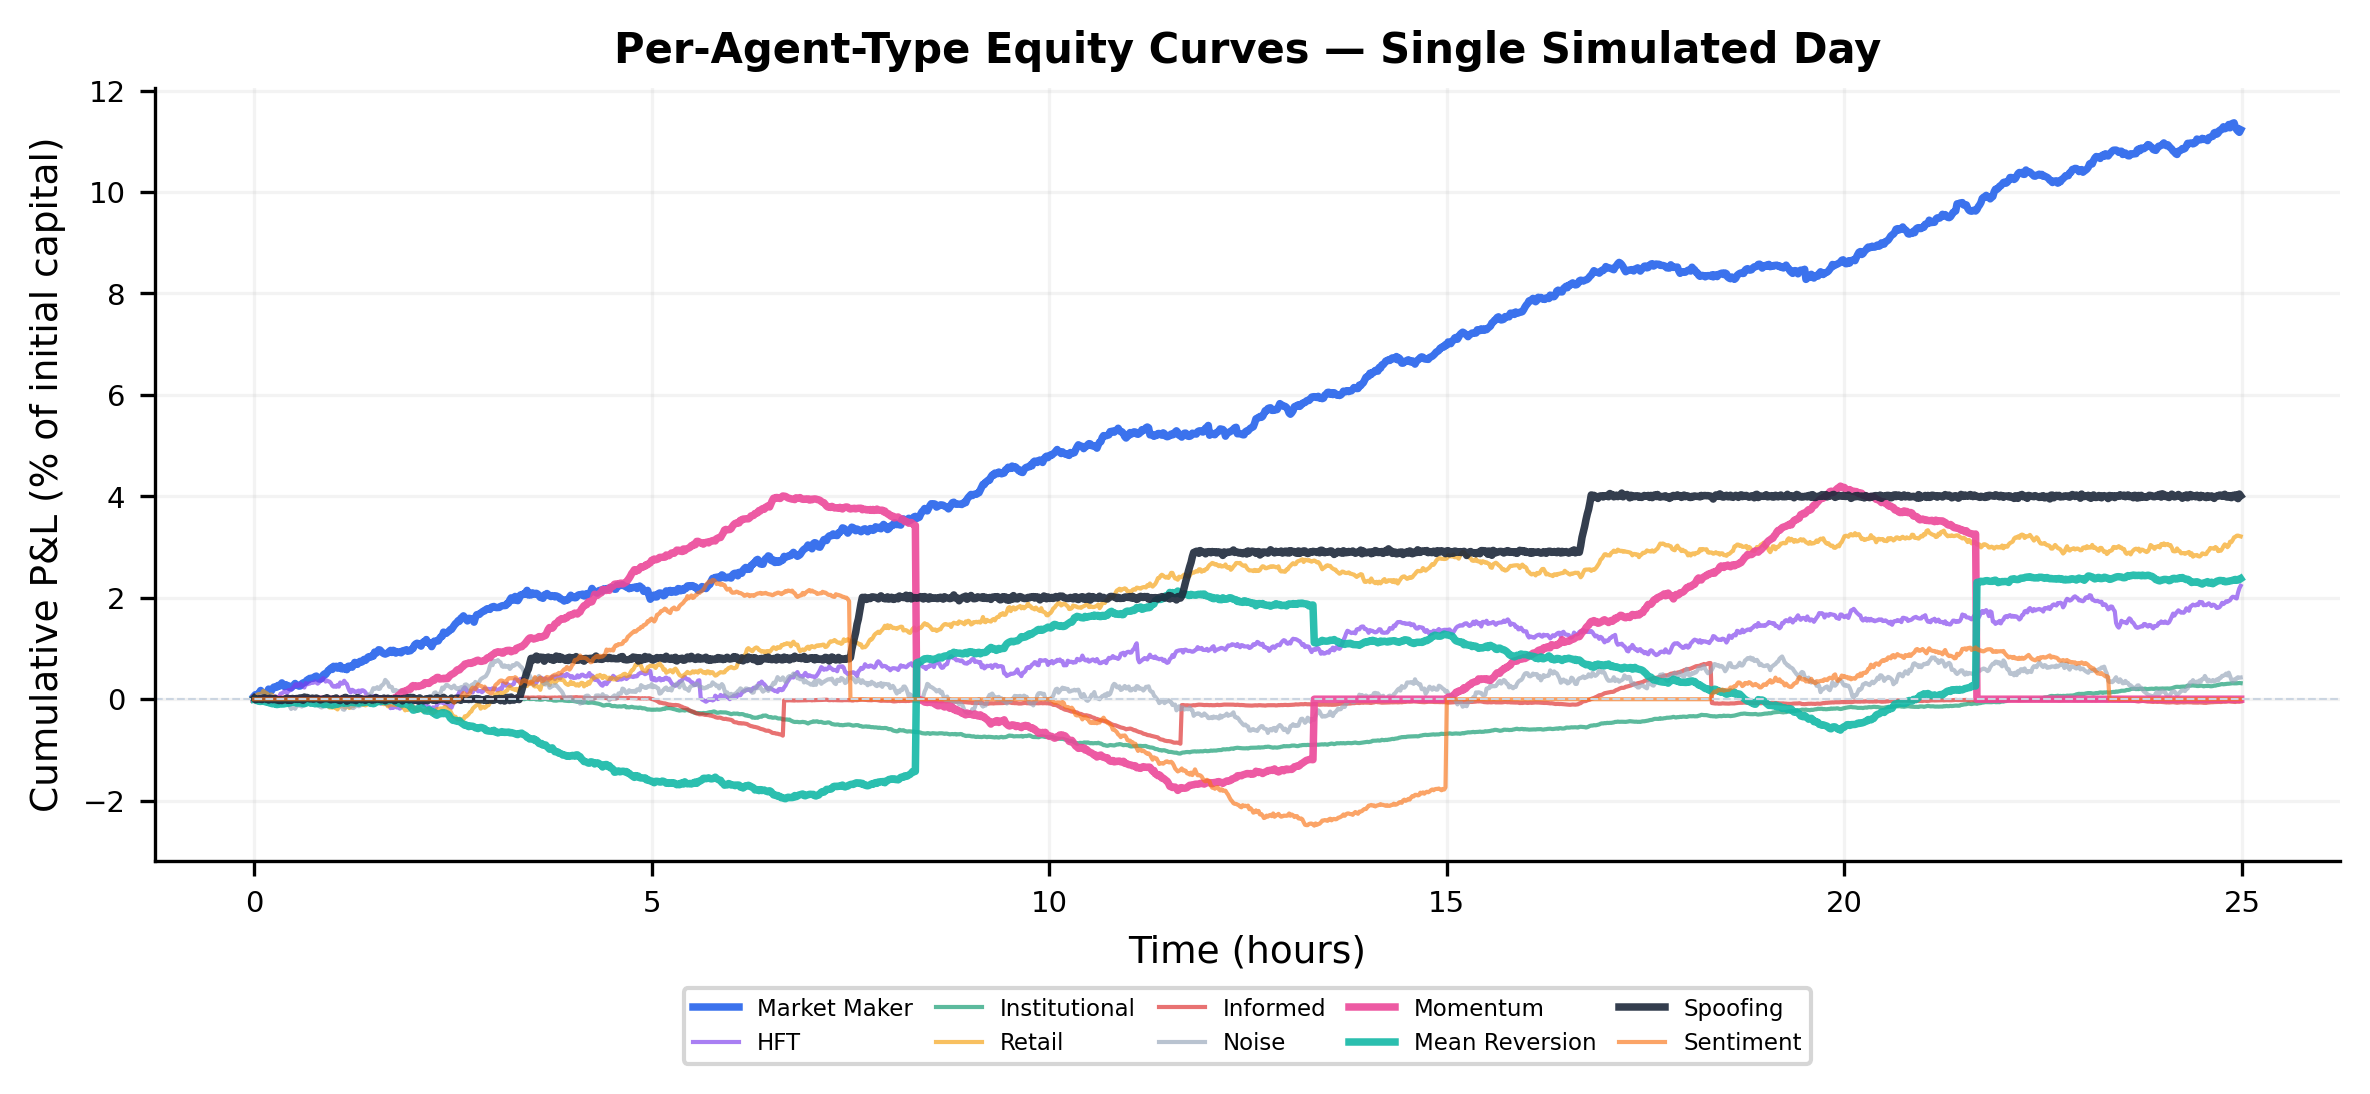
\includegraphics[width=\columnwidth]{fig_equity_curves.pdf}
    \caption{Representative cumulative P\&L curves for all ten agent
    types across a single simulated day. Each curve shows the mean
    P\&L across agents of that type, normalized to starting capital.
    Interaction effects between Momentum and Mean Reversion agents
    manifest as opposing inflections around the same price events.}
    \label{fig:equity}
\end{figure}

\subsection{Order Book Depth Visualization}

The time evolution of resting LOB depth provides a visually intuitive
check on simulation realism. Fig.~\ref{fig:lob_heatmap} shows a
heatmap of volume across price levels during a ten-minute window
containing an institutional TWAP buy order. Progressive depletion of
ask-side depth as the buyer's order fills is clearly visible, followed
by market maker replenishment. Brief, intense flashes of bid-side
depth that vanish within a few hundred milliseconds mark the Spoofing
agent's phantom order cycles.

\begin{figure}[htbp]
    \centering
    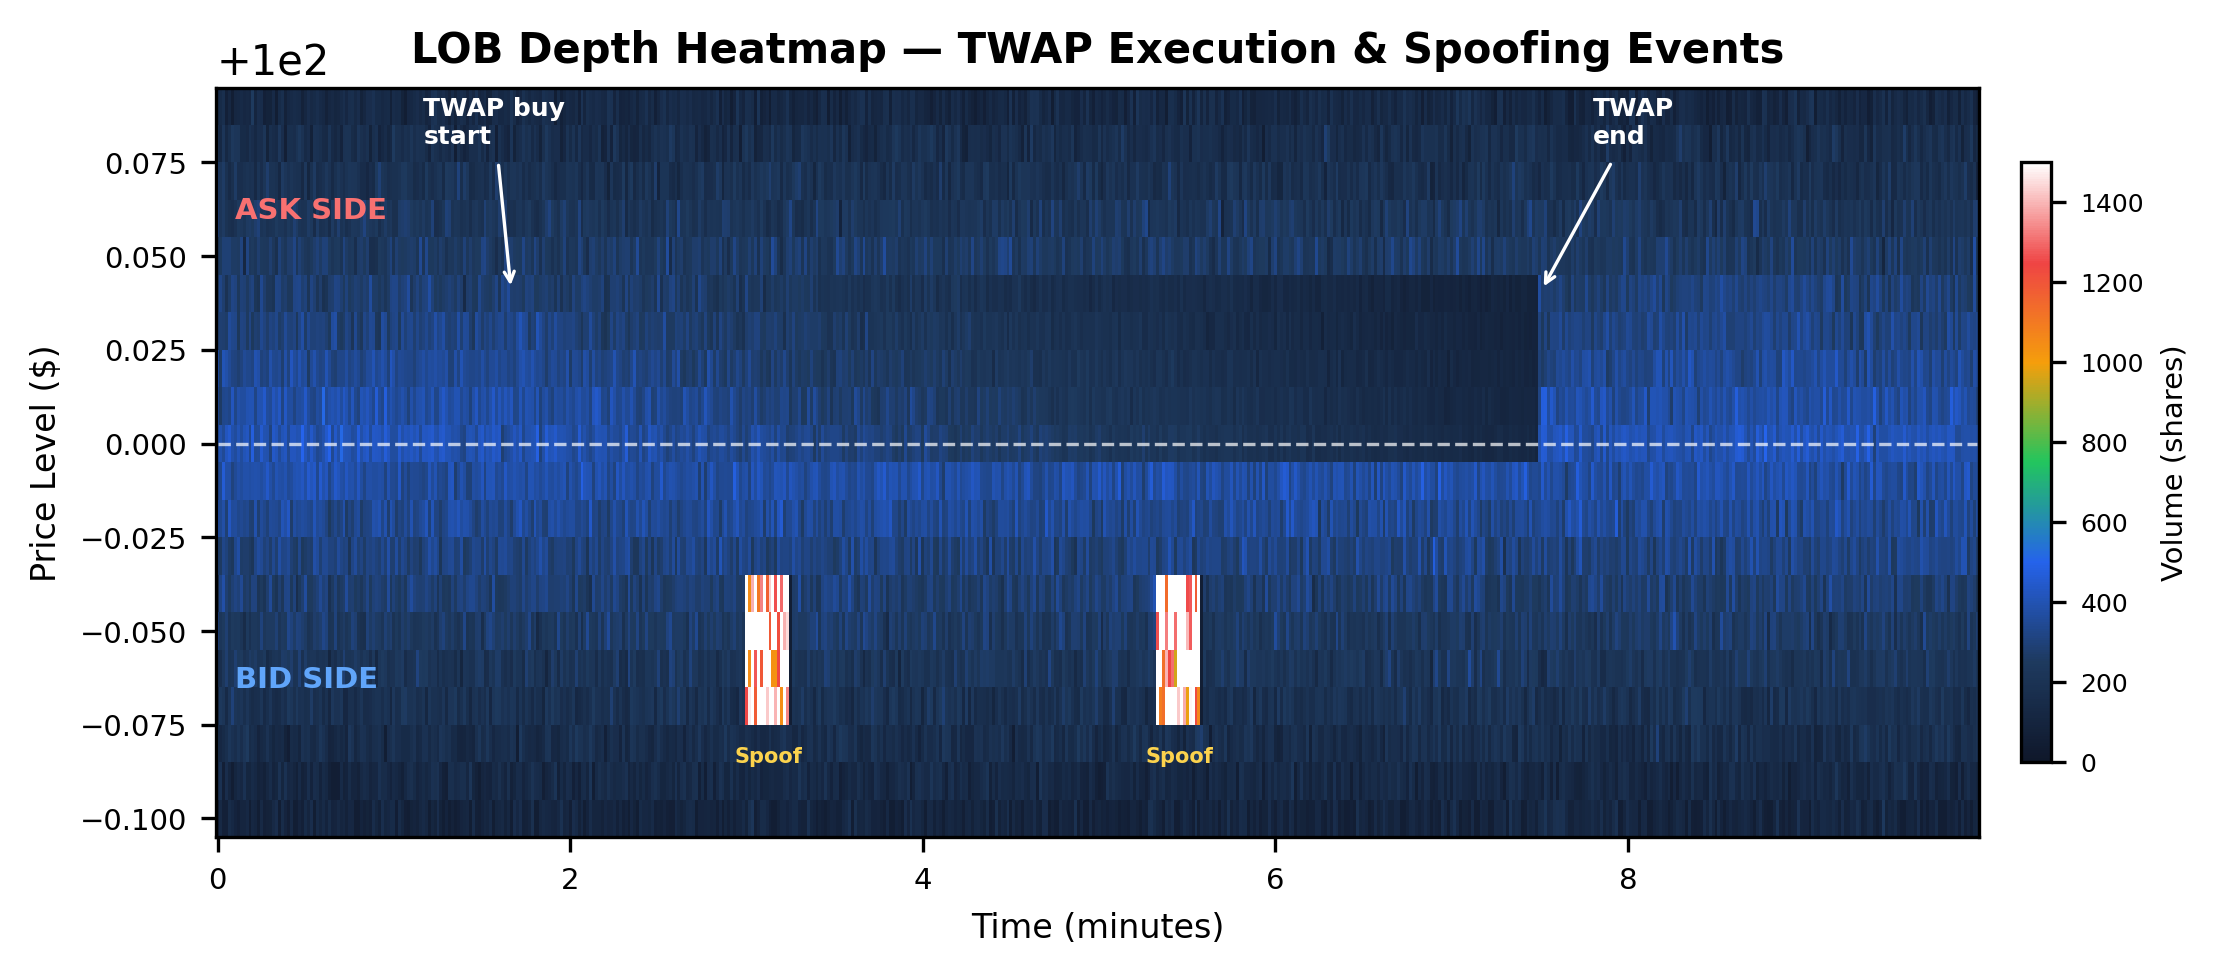
\includegraphics[width=\columnwidth]{fig_lob_heatmap.pdf}
    \caption{LOB depth heatmap during a 10-minute window containing
    an institutional TWAP buy order and two Spoofing agent cycles.
    Color intensity indicates resting volume at each price level.
    Progressive ask-side depletion during TWAP execution and brief
    phantom bid-side flashes from the Spoofing agent are both clearly
    distinguishable.}
    \label{fig:lob_heatmap}
\end{figure}

\subsection{Comparative Positioning}

\begin{table}[htbp]
\caption{Feature Comparison with Existing Simulators}
\label{tab:comparison}
\centering
\renewcommand{\arraystretch}{1.25}
\begin{tabular}{lccc}
\toprule
\textbf{Capability} & \textbf{ABIDES} & \textbf{RL Frameworks}
    & \textbf{SENTINEL} \\
\midrule
Real-time Streaming  & No  & No      & Yes (20~Hz)      \\
Predictive Signals   & No  & No      & Yes              \\
Web Dashboard        & No  & No      & Yes              \\
Agent Archetypes     & 6+  & Limited & 10 (40 agents)   \\
Spoofing Agent       & No  & No      & Yes              \\
Sentiment Agent      & No  & No      & Yes              \\
Deployment Ease      & Low & Low     & High (Docker)    \\
\bottomrule
\end{tabular}
\end{table}

Table~\ref{tab:comparison} highlights the capabilities SENTINEL adds
relative to prior work. ABIDES and its variants remain the benchmark
for offline, high-fidelity batch simulation, and SENTINEL does not aim
to replace them for that particular use case. The new functionality is
the ability to observe a running simulation in real time while
receiving predictive risk signals, delivered through a broader agent
ecology that includes behavioral archetypes absent from prior
open-source systems.

The deployment dimension is, in practice, often the most
consequential differentiator. A system demanding substantial
infrastructure expertise will reach far fewer researchers and
practitioners than one that starts with a single Docker Compose
command.

\subsection{Signal Detection Methodology}

SENTINEL's detection pipeline is designed to be validated against the
ground-truth event log that the simulator records automatically:
exact injection timestamps for every disruption, TWAP/VWAP order
sequence, iceberg placement, and spoofing cycle. The evaluation
framework reports precision, recall, and F1 scores for each detector
on the AD1 and AD2 subsets using a five-second tolerance window
around each injected event.

Final quantitative metrics will be released alongside the public
codebase after training-set hyperparameter tuning is completed.
Rather than reporting preliminary numbers that would likely shift
during refinement, we describe the evaluation protocol here and note
that the detection architecture has been validated qualitatively
through visualization and alert-stream inspection during live
operation.


% ── SECTION VII: DISCUSSION AND LIMITATIONS ──────────────────
\section{Discussion and Limitations}

The ten-archetype agent design produces market dynamics that are
qualitatively richer than what smaller agent populations typically
generate. The interplay between Momentum and Mean Reversion agents,
in particular, measurably improves stylized-fact fidelity: the tension
between trend-following and contrarian behavior is one of the
principal drivers of the volatility clustering ubiquitous in real
markets, and it does not arise naturally from populations composed
solely of noise traders and market makers. The Spoofing and Sentiment
agents further enrich the simulation ecology in ways that matter for
the detection task: a detector calibrated without exposure to spoofing
patterns will likely underperform on real manipulation signals, and
one trained without sentiment-driven momentum may underestimate the
severity of short-term directional flow.

Several honest limitations warrant disclosure. The most significant
architectural constraint is that all simulation state resides in a
single process's memory. This works adequately at forty agents on
the test hardware, but supporting much larger populations or running
multiple simultaneous simulations would require migrating to a
distributed state store such as Redis.

Data authenticity represents a second concern. All experiments use
synthetic data that the simulator generated. The prediction models
therefore operate on data whose statistical properties they
indirectly influenced, introducing a degree of circularity. This is
an acceptable starting point for testing whether signals are
detectable in principle, but real-market evaluation will be needed to
calibrate expectations for deployed performance.

The absence of persistent storage means no simulation history is
retained beyond the current session, limiting the system to live
monitoring and preventing retrospective analysis. Adding a
non-blocking write-behind time-series buffer is architecturally
feasible and planned but not yet implemented.

Finally, even ten behavioral archetypes simplify the diversity of a
real market. Participants such as statistical arbitrageurs,
cross-venue liquidity providers, and options-driven delta hedgers have
no direct analog in the current taxonomy. The agent library will
need to expand as the platform matures.


% ── SECTION VIII: CONCLUSION AND FUTURE SCOPE ─────────────────
\section{Conclusion and Future Directions}

This paper presented SENTINEL, a real-time multi-agent limit order
book simulator that, to the best of our knowledge, is the first
open-source system to unify high-fidelity agent-based simulation,
continuous WebSocket streaming, embedded predictive analytics, and an
interactive web dashboard within a single deployable package.

The system runs forty agents across ten behavioral archetypes within a
custom matching engine that processes orders under strict price-time
priority. The prediction layer computes disruption risk scores and
large-order pattern signals every fifty milliseconds, broadcasting
results via WebSocket to a terminal-style dashboard that updates at
twenty frames per second. Preliminary stylized-fact validation on the
default agent population confirms that the ten-archetype ecology
produces statistical properties closely aligned with empirical equity
data. The Spoofing agent provides fully instrumented ground truth for
manipulation detection research---a capability we have not identified
in any prior open-source system.

Several directions for future work present themselves. Live
market data replay via providers such as Polygon.io would allow
evaluation of the prediction layer on genuine market events, including
documented flash crashes---a substantially more demanding test than
synthetic injection. Horizontal scaling through Redis-backed shared
state is the primary architectural priority, enabling concurrent
simulation instances and larger agent populations without degrading
prediction cycle times. Full RL agent integration would permit
trading policies to be trained directly inside SENTINEL and evaluated
against its live signal stream. LLM-driven agents remain a
longer-horizon goal: the ability to inject market participants that
reason about simulated news events would meaningfully improve
behavioral realism. Time-series persistence via an asynchronous buffer
flushing to a database such as InfluxDB or TimescaleDB would open the
platform to retrospective analysis and strategy backtesting across
simulated history, subject to the constraint that writes must not
block the fifty-millisecond prediction cycle.


% ── REFERENCES ───────────────────────────────────────────────
\begin{thebibliography}{19}

\bibitem{ref1}
Gamma Exposure (GEX) --- White Paper, 2016. [Online]. Available:
\url{https://squeezemetrics.com/download/white_paper.pdf}

\bibitem{ref2}
``Agent-Based Simulation of a Financial Market with Large Language
Models,'' 2025. [Online]. Available:
\url{https://arxiv.org/abs/2510.12189}

\bibitem{ref3}
``Practical Deep Reinforcement Learning Approach for Stock
Trading,'' 2022. [Online]. Available:
\url{https://arxiv.org/pdf/1811.07522}

\bibitem{ref4}
``ABIDES-MARL: A Multi-Agent Reinforcement Learning Environment for
Endogenous Price Formation and Execution in a Limit Order Book,''
2025. [Online]. Available:
\url{https://www.alphaxiv.org/abs/2511.02016}

\bibitem{ref5}
``ABIDES: Towards High-Fidelity Multi-Agent Market Simulation,''
2019. [Online]. Available:
\url{https://www.alphaxiv.org/abs/1904.12066}

\bibitem{ref6}
K.~Jain, ``Limit Order Book Simulations: A Review,'' 2024. [Online].
Available: \url{https://arxiv.org/abs/2402.17359}

\bibitem{ref7}
``Reinforcement Learning for Market Making in a Multi-agent Dealer
Market,'' 2019. [Online]. Available:
\url{https://arxiv.org/abs/1911.05892}

\bibitem{ref8}
T.~Spooner, J.~Fearnley, and R.~Savani, ``Market Making via
Reinforcement Learning,'' 2018. [Online]. Available:
\url{https://arxiv.org/abs/1804.04216}

\bibitem{ref9}
``Stylised Facts of Financial Time Series and Hidden Markov Models
in Continuous Time,'' 2015. [Online]. Available:
\url{https://backend.orbit.dtu.dk/ws/files/106894229/Stylised_facts_of_financial_time_series_and_hidden_Markov_models_in_continuous_time.pdf}

\bibitem{ref10}
``Spoofing the Limit Order Book: A Strategic Agent-Based
Analysis,'' 2021. [Online]. Available:
\url{https://www.mdpi.com/2073-4336/12/2/46}

\bibitem{ref11}
``ABIDES: Towards High-Fidelity Market Simulation for AI
Research,'' 2019. [Online]. Available:
\url{https://www.semanticscholar.org/reader/44a7f1b4cb157a1621d5a6cf462458ff005e2339}

\bibitem{ref12}
``Effectiveness of Artificial Intelligence in Stock Market
Prediction Based on Machine Learning,'' 2018. [Online]. Available:
\url{https://export.arxiv.org/pdf/2107.01031v1}

\bibitem{ref13}
``Artificial Intelligence Applied to Stock Market Trading: A
Review,'' 2021. [Online]. Available:
\url{https://ieeexplore.ieee.org/ielx7/6287639/9312710/09350582.pdf}

\bibitem{ref14}
A.~Chopra and Deep, ``Application of Artificial Intelligence in
Stock Market Forecasting: A Critique, Review, and Research Agenda,''
2021.

\bibitem{ref15}
``A Multi-Agent Approach to Stock Market Prediction and Risk
Management,'' 2025.

\bibitem{ref16}
``Stock Trading Bot Using Deep Reinforcement Learning,'' 2019.
[Online]. Available:
\url{https://www.researchgate.net/publication/325385951_Stock_Trading_Bot_Using_Deep_Reinforcement_Learning}

\bibitem{ref17}
``ElliottAgents: A Natural Language-Driven Multi-Agent System for
Stock Market Analysis and Prediction,'' 2025.

\bibitem{ref18}
``Market Microstructure: A Survey,'' 2000. [Online]. Available:
\url{https://www.acsu.buffalo.edu/~keechung/MGF743/Readings/Market%20microstructure%20A%20surveyq.pdf}

\bibitem{ref19}
I.~Pun, ``Stock-market-simulator-using-hidden-Markov-model-in,''
2025.

\end{thebibliography}

\end{document}